\documentclass[acmtog]{acmart}
\usepackage{graphicx}
\usepackage{subfigure}
\usepackage{natbib}
\usepackage{listings}
\usepackage{bm}
\usepackage{amsmath}
\usepackage{listings}
\usepackage{animate}

\lstset{
	showstringspaces=false,
	showspaces=false
}

\definecolor{blve}{rgb}{0.3372549 , 0.61176471, 0.83921569}
\definecolor{gr33n}{rgb}{0.29019608, 0.7372549, 0.64705882}
\makeatletter
\lst@InstallKeywords k{class}{classstyle}\slshape{classstyle}{}ld
\makeatother
\lstset{language=C++,
	basicstyle=\ttfamily,
	keywordstyle=\color{blve}\ttfamily,
	stringstyle=\color{red}\ttfamily,
	commentstyle=\color{magenta}\ttfamily,
	morecomment=[l][\color{magenta}]{\#},
	classstyle = \bfseries\color{gr33n}, 
	tabsize=2
}
\lstset{basicstyle=\ttfamily}

% Title portion
\title{Final Report:\\ {}} 

\author{Huang Kuan \quad student NO.:\quad 2020533123
	\quad email:\quad huangkuan@shanghaitech.edu.cn}

\author{\\Yin Hairui \quad student NO.:\quad 2020533028
	\quad email:\quad yinhr@shanghaitech.edu.cn}

% Document starts
\begin{document}
\maketitle

\vspace*{2 ex}

\section{Introduction}
SPH, which stands for Smoothed Particle Hydrodynamics, is a basic liquid fluid simulation approach. It is a Lagrangian method that can be used to model fluid flow by treating each particle as a discrete element. \\
Each SPH fluid particle is seen as a discrete fluid unit. The motion of fluid particles is affected by the other ones within a smooth radius. The extent to which one particle influences another depends on the smoothing kernel, which is a function of one variable dependent on the radius. Since the SPH method is a pure Lagrangian method, the motion of the particle is based on the current acceleration value at a certain time. The acceleration of a particle takes into account the density, pressure and relative velocity of the particles around it. \\
In our implementation, the 3 following parts have been successfully deployed:
\begin{itemize}
\item WCSPH Solver
\item PCISPH Solver
\item Visualization
\end{itemize}

\section{Previous Work}
In others' previous work, Weakly compressible SPH for free surface flows by Markus Becker Matthias Teschner is raised, which can deal with the pressure force and viscosity force of a particle system but has a maximum time step limitation.
And named "Predictive-Corrective Incompressible SPH", B. Solenthaler and R. Pajarola proposed a novel, fully Lagrangian, incompressible SPH method featuring the advantages of both WCSPH and ISPH in one model, namely low computational cost per physics update and large time steps. Their method makes use of a prediction-correction scheme which propagates the estimated density values through the fluid and updates the pressures in such a way that incompressibility is achieved. The propagation stops as soon as a previously userdefined density variation limit is reached for each individual particle. They showed that their new predictive-corrective incompressible SPH (PCISPH) method outperforms WCSPH by more than an order of magnitude while the computations are in good agreement with the WCSPH results. The efficiency of their method enables an animator to produce high-resolution fluid animations within reasonable time without compressibility artifacts.

\section{WCSPH Solver}
This section provides the implementation details of the whole SPH fluid simulation and covers governing equations, time step calculations, and object-fluid interaction methods.

\subsection{Governing Equations}
In order to find the acceleration of a particle, the density and pressure values must be calculated. The following equation is the sum of the nearest neighbor masses of a particle weighted by the kernel function.
\begin{equation*}
	p_i = \sum_{j} m_j W_{ij}
\end{equation*}
Where $p$ is density, $m$ is mass, $W$ is the Poly6 smoothing kernel:
\begin{equation*}
	W_{ij}=\frac{315}{64\pi h^9}(h^2-r^2)^3
\end{equation*}
Where h is the smoothing radius which is set to 0.2 by default, r is the distance between 2 involved particles. This formula preserves the square form and eliminates the operation of calculating the square root through deformation, which greatly reduces the amount of computation. \\
After the density of a particle is figured out, the pressure can now be computed as follows:
\begin{equation*}
	P = K(p-p_0)
\end{equation*}
Where $P$ is the pressure, $K$ is the pressure constant which is set to 20 by default, $p$ is the density of the particle, $p_0$ is the reference density which is set to 40 by default. When the actual density is less than the reference density, force it to be equal to the reference density to avoid negative values. \\
With the computing results, the The acceleration of a particle can now be computed as follows:
\begin{equation*}
	a_i = -\sum_{j} \frac{m_j}{m_i} \frac{P_i+P_j}{2 p_i p_j}W_{ij} \hat{r}_ij
\end{equation*}
Where $a$ is the particle acceleration, $P_i$ and $P_j$ are the pressure of the involved particles, $\hat{r}_ij$ is the normalized vector of the position of particle $j$ to particle $i$, $W_{ij}$ is the gradient form of Spiky kernel smoothing function which can be presented as follows:
\begin{equation*}
	W_{ij} = -\frac{45}{\pi h^6} (h-r)^2
\end{equation*}
The acceleration described above is caused by the mass, density and pressure of the neighbor particles. To dampen the motion of the system, a viscosity term can be applied to the acceleration according to the following formula:
\begin{equation*}
	a_{vi} = \lambda \sum_{j} \frac{1}{p_j} (v_j-v_i) (-W_{ij}) (h-r)
\end{equation*}
Where $a_{vi}$ is the viscosity acceleration, $\lambda$ is the viscosity constant which is set to 0.018 by default, $v_i$ and $v_j$ are the velocity of the involved particles. In addition, $W_{ij}$, $h$ and $r$ have the same meanings as the ones presented before. Besides, the acceleration due to the force of gravity should also be added.

\subsection{Time Step Calculation}
The goal of choosing a time step is to choose a maximum value so that a particle will move less than a smoothing radius in a time step. The following formula is used to calculate the next time step in this implementation:
\begin{equation*}
	\Delta t = max\{ \frac{Ch}{v_{max}}, \sqrt{\frac{h}{a_{max}}}, \frac{Ch}{c_{max}} \}
\end{equation*}
Where $v_{max}$ is the maximum velocity in the particle system, $a_{max}$ is the maximum acceleration in the particle system, $c_{max}$ is the maximum speed of sound, $C$ is the Courant safety constant which is set to 1.0 by default. The speed of sound can be calculate as follows:
\begin{equation*}
	c = \sqrt{\frac{\gamma P}{p}}
\end{equation*}
Where $c$ is the speed of sound, $\gamma$ is the ratio of specific heats which is set to 1.0 by default.\\
In our implementation, since we have set a maximum velocity of particle to be 75, we can directly find the $\frac{Ch}{v_{max}}$ part. However, the maximum time limitation is too small so we still use a fixed frame update rate between two intervals in the main function.
The method is simple, but the results are still acceptable, and can present the practical situation of fluid motion.

\subsection{Object-Fluid Interaction}
Object-fluid interaction is handled in the following specific approach. The static fluid boundaries are handled with planes that the particles cannot intersect. The boundary planes are given a repulsive force in the direction of their normals to push away particles that are too close to the boundary. If a particle hits a boundary, the velocity of it is adjusted so that it bounces off the surface.

\section{PCISPH Solver}
\subsection{Main Idea}
To avoid the time step restriction of WCSPH we propose to use a prediction-correction scheme based on the SPH algorithm (PCISPH). In our method, the velocities and positions are temporarily forwarded in time and the new particle densities are estimated.
Then, for each particle, the predicted variation from the reference density is computed and used to update the pressure values, which in turn enter the recomputation of the pressure forces. Similar to a Jacobi iteration for linear systems, this process is iterated until maxIteration. Note that this is a nonlinear problem since we include collision handling and updated kernel values in our iteration process. As a final step, the velocities and positions of the next physics update step are computed.

\subsection{Force and Delta x Computation}
First, we still use the WCSPH method to compute the pressure and pressure force $F^{v,g,ext}$ combined with viscosity force and gravity. And the position relationship between time $t$ and time $t+1$ is:
$$
 x(t)+\Delta x(t)=x(t+1)
$$
We are required to find the $\Delta x_i$ which is used to predict the next time pressure.
$$
\Delta x_i = \Delta t^2\frac{F^{v,g,ext}}{m}
$$


\subsection{Delta Density Computation}
The Density between time $t$ and time $t+1$ has the following relationship, where we use the first order Taylor approximation to approximate the relationship
\begin{equation*}
	\begin{aligned}
		\rho_i(t+1)&=m\sum_j W(d_{ij}(t))+\nabla W(d_{ij}(t))\cdot \Delta d_{ij}(t)\\
		&=m\sum_j W(x_i(t)-x_j(t))+\\
		&m\sum_j \nabla W(x_i(t)-x_j(t))\cdot(\Delta x_i(t)-\Delta x_j(t))\\
		&=\rho_i(t)+\Delta \rho_i(t)
	\end{aligned}
\end{equation*}
\newline
In this equation, the term $\Delta \rho_i(t)$ is unknown and, as we show later, a function of $p$ which we are looking for. After reformulation and using $W_{ij}= W(x_i(t)-x_j(t))$, we get
\begin{equation*}
	\Delta \rho_i(t)=m\sum_j \nabla W_{ij}\cdot(\Delta x_i(t)-\Delta x_j(t))
\end{equation*}


\subsection{Pressure Correctness}
Considering the pressure between time $t$ and time $t+1$, since the time step is very small, the average pressure will not change to a large extent. Defining the average pressure to be $\tilde{p_i}$, and the average pressure of a particle is needed to achieve a change in density of $\Delta \rho_i(t)$:
\begin{equation*}
	\tilde{p_i}=\frac{\Delta \rho_i(t)}{\beta(-\sum_j\nabla W_{ij}\cdot \sum_j\nabla W_{ij}\cdot-\sum_j(\nabla W_{ij}\cdot \nabla W_{ij}))}
\end{equation*}
where $\beta$ is
\begin{equation*}
	\beta=\Delta t^2 m^2 \frac{2}{\rho_0^2}
\end{equation*}
Since we repeat the prediction-correction step as long as the incompressibility condition is not yet satisfied, the correction pressures of the individual iterations are accumulated as:
\begin{equation*}
	p_i+=\tilde{p_i}
\end{equation*}

\subsection{Compute New Force}
Within the updated pressure, we can compute the revise force of pressure force with the same step in WCSPH.

\subsection{Loop Within limitation}
In the paper of PCISPH algorithm, they consider both $\rho_{err}(t+1)$ and iteration time to jump out of loop between Step 4.2 to Step 4.5 with the pseudocode: $\rho_{err}(t+1) > eta\ ||\ (iter < minIterations)$.\\ However, to simplify the computation, we iterate the same maximum amount of time(set to be three) to finish the loop.

\section{Visualization}
With the help of our homework 5 code, we present fluid particles in the form of colored balls, and at the same time provide the observer with a camera that can freely move and turn the angle of view, thus achieving a great effect of visualization.

\section{Results}
After successfully implementing the 3 basic parts, the simulation now has a neat look. The following screenshots is captured in the correct time order. For a more complete demonstration, check out the demo video or run the program locally.
\begin{figure}[h]
	\centering
	\subfigure[]
	{
		\begin{minipage}[b]{.4\linewidth}
			\centering
			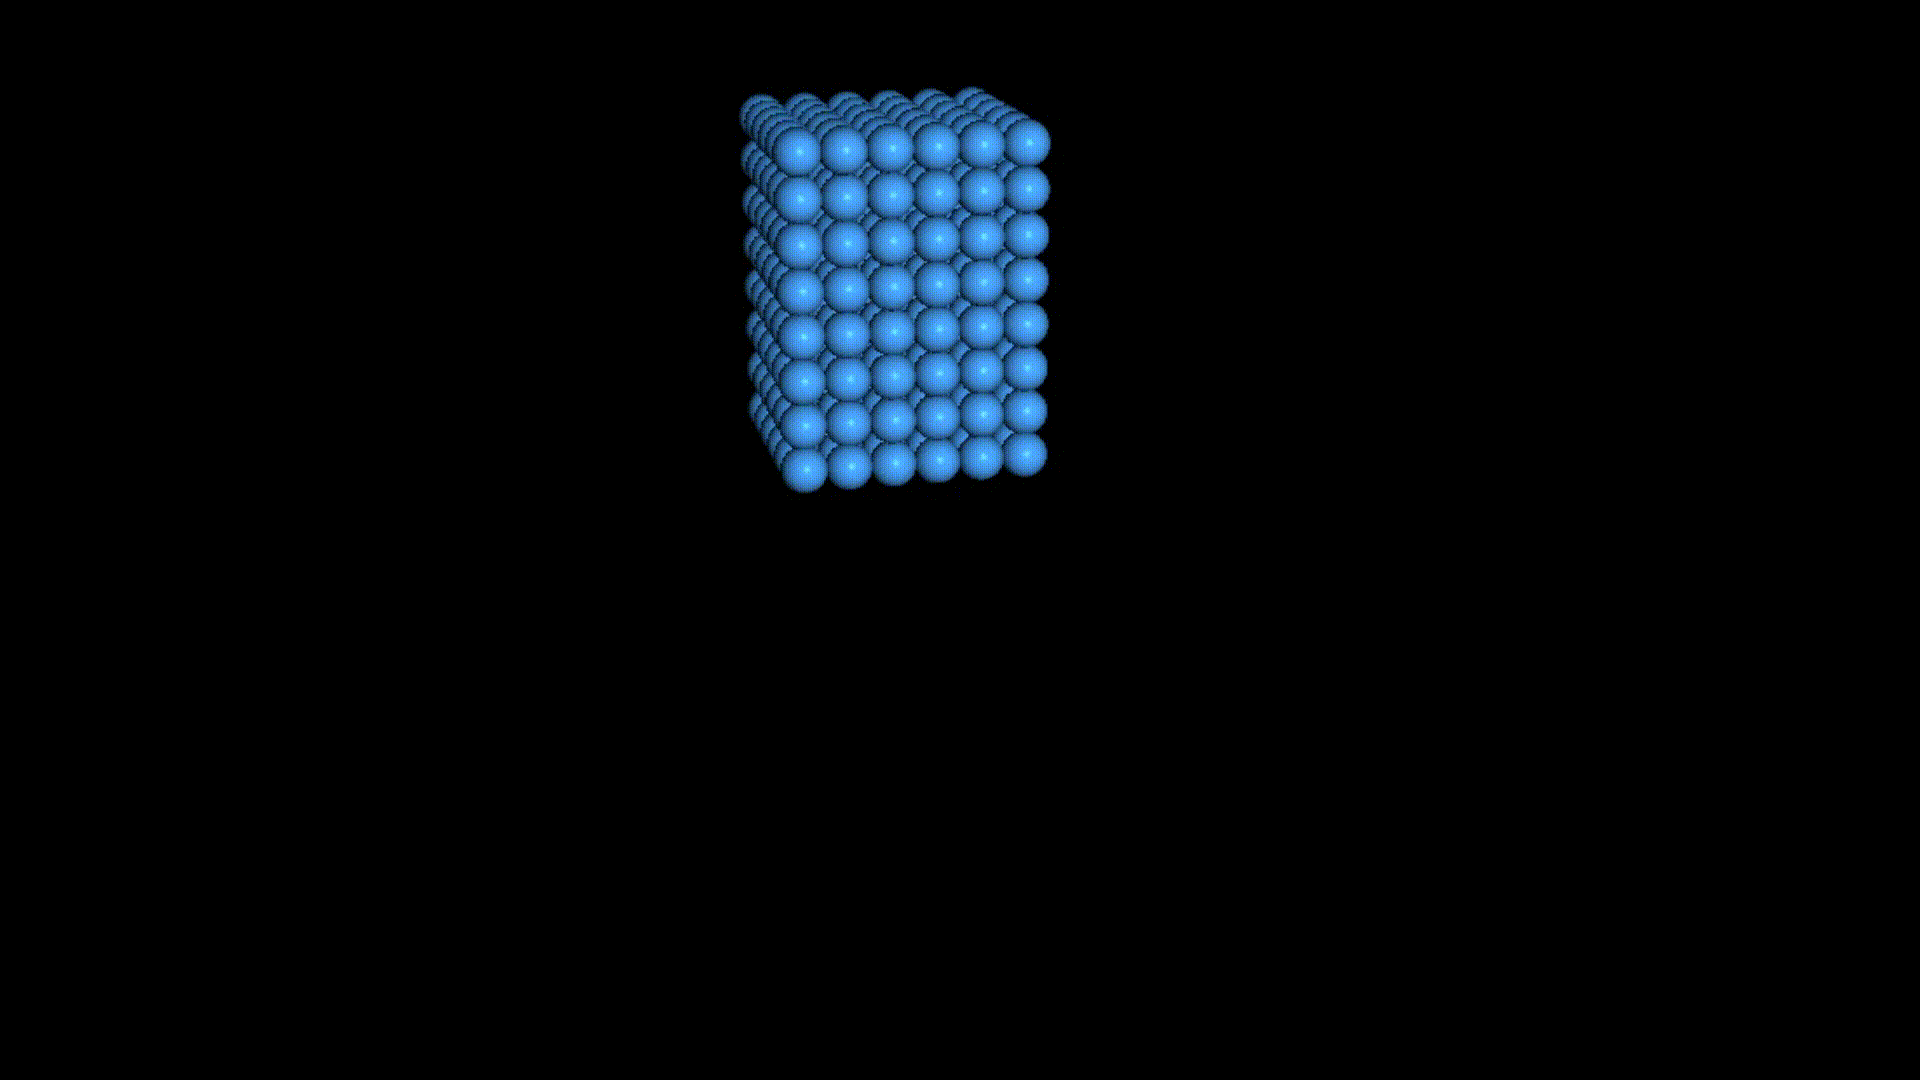
\includegraphics[scale=0.05]{image/image-0.png}
		\end{minipage}
	}
	\subfigure[]
	{
		\begin{minipage}[b]{.4\linewidth}
			\centering
			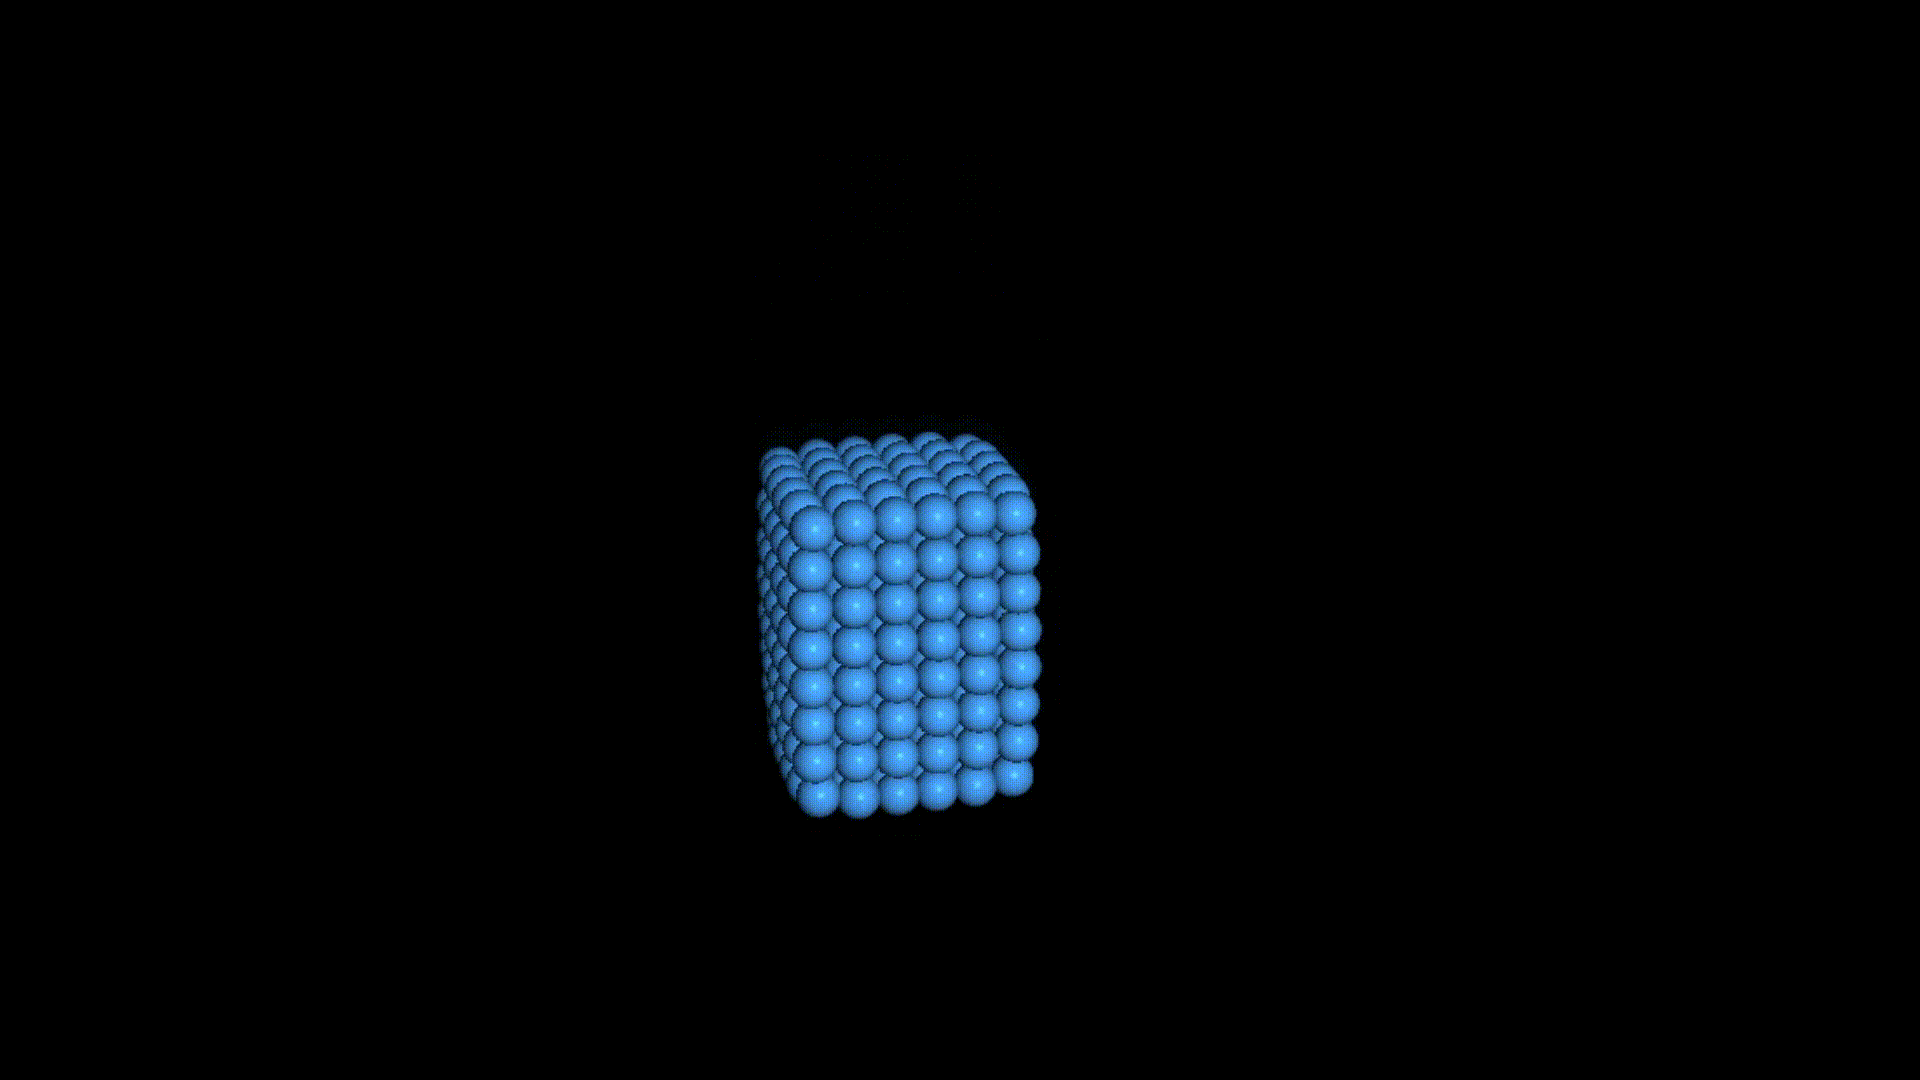
\includegraphics[scale=0.05]{image/image-1.png}
		\end{minipage}
	}
\end{figure}
\begin{figure}[h]
	\centering
	\subfigure[]
	{
		\begin{minipage}[b]{.4\linewidth}
			\centering
			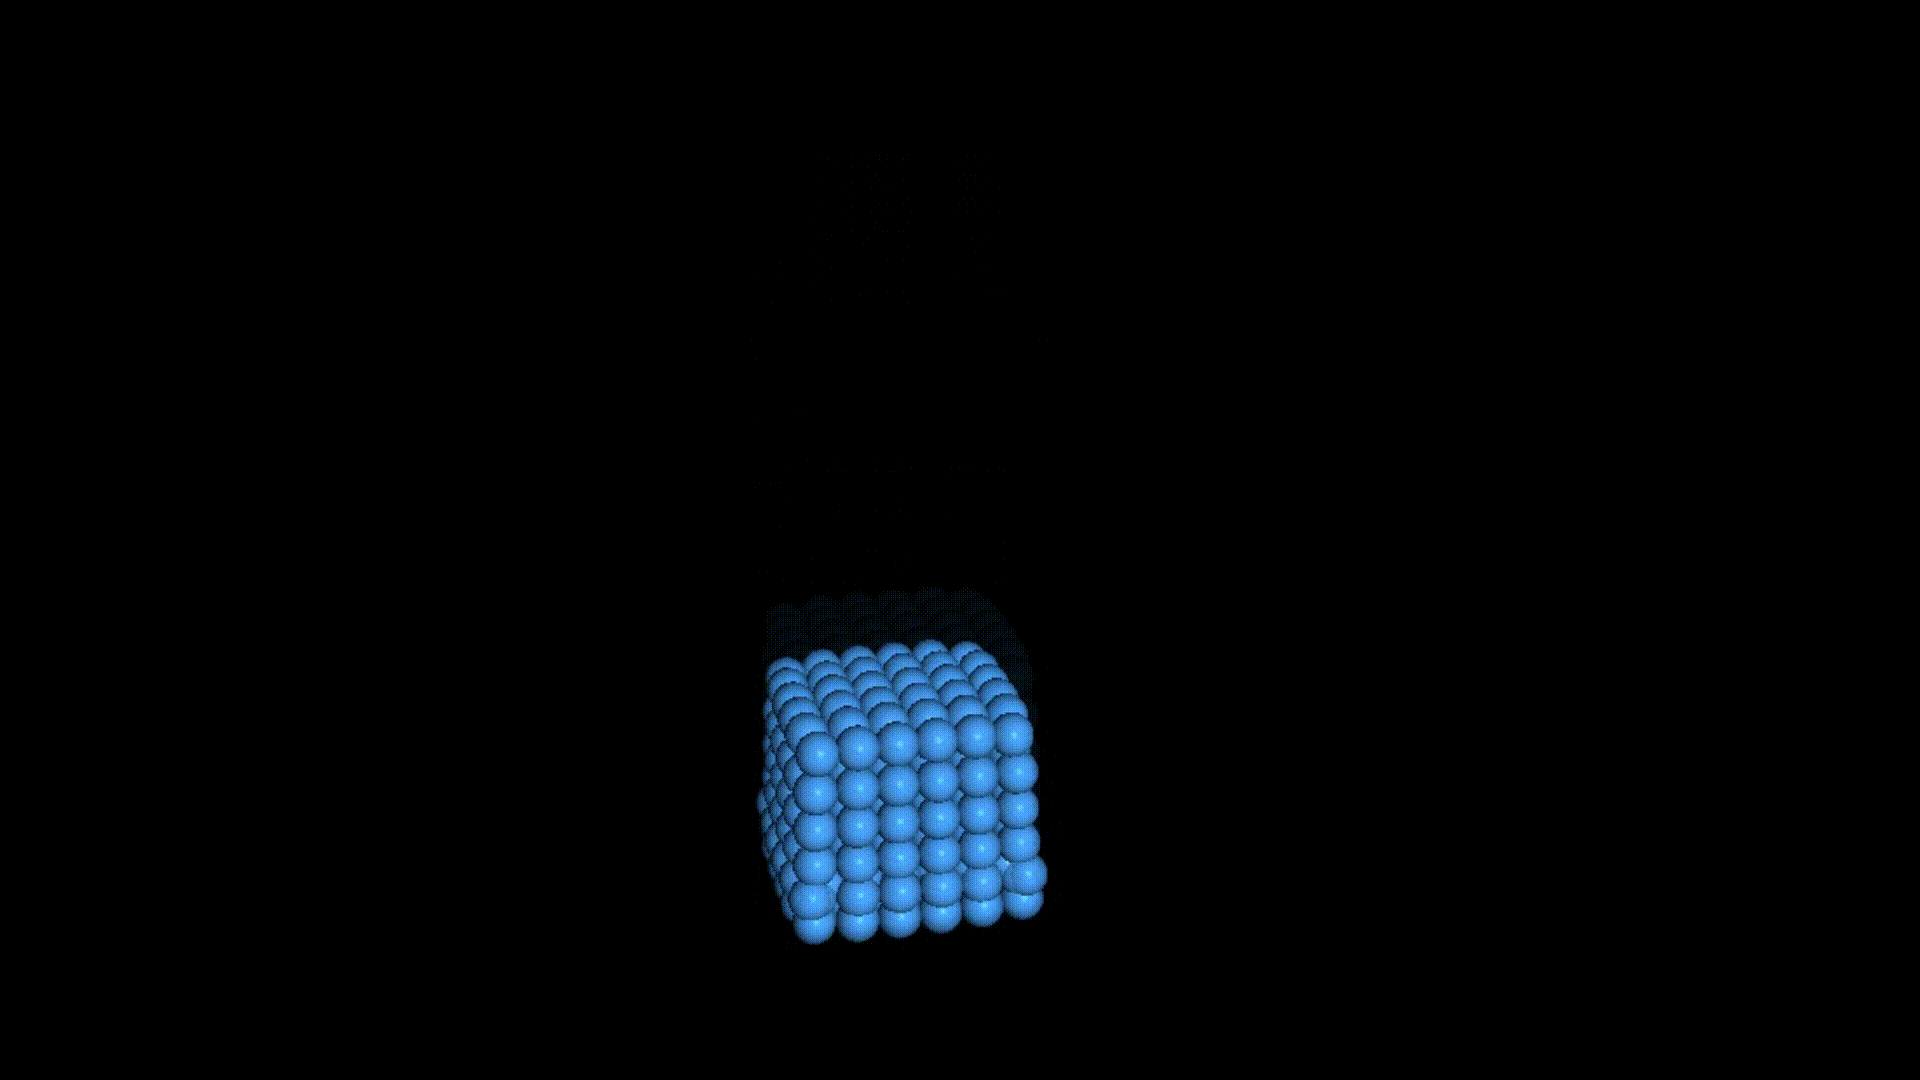
\includegraphics[scale=0.05]{image/image-2.png}
		\end{minipage}
	}
	\subfigure[]
	{
		\begin{minipage}[b]{.4\linewidth}
			\centering
			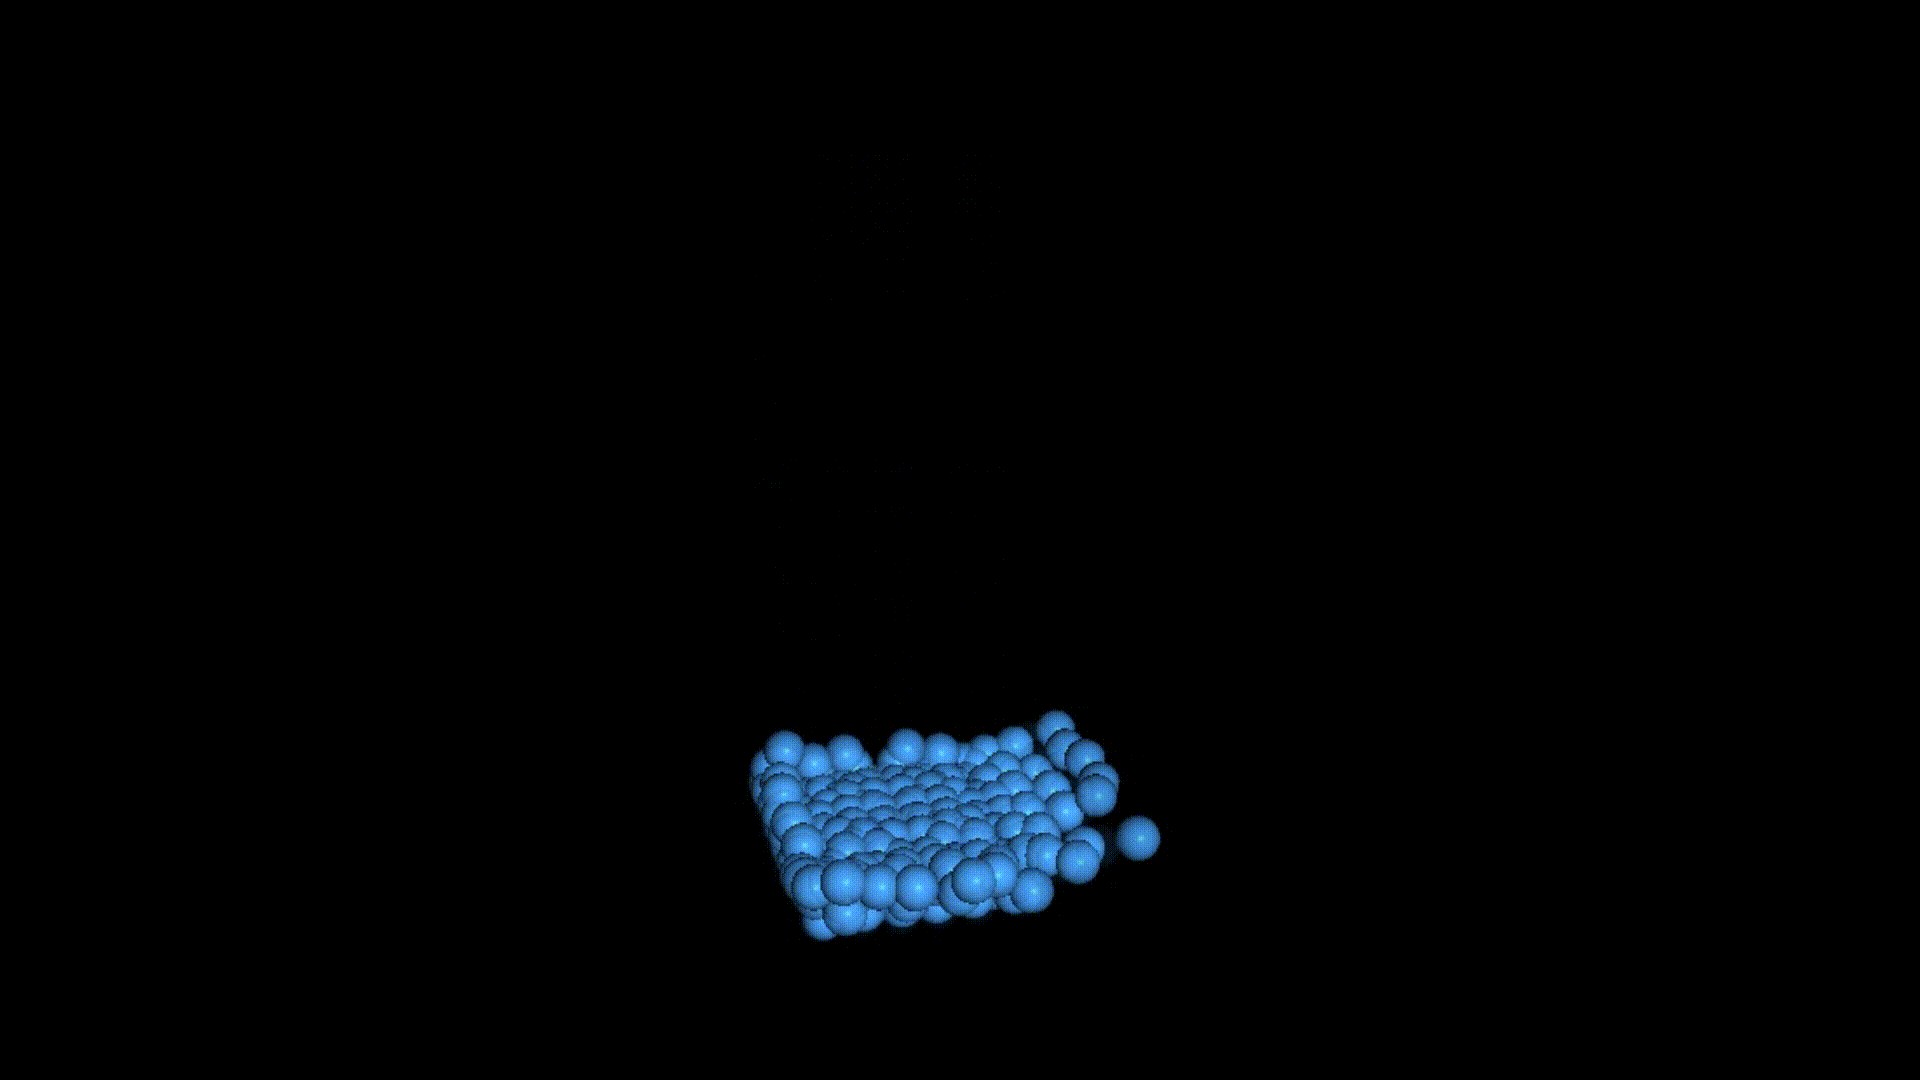
\includegraphics[scale=0.05]{image/image-3.png}
		\end{minipage}
	}
\end{figure}
\begin{figure}[h]
	\centering
	\subfigure[]
	{
		\begin{minipage}[b]{.4\linewidth}
			\centering
			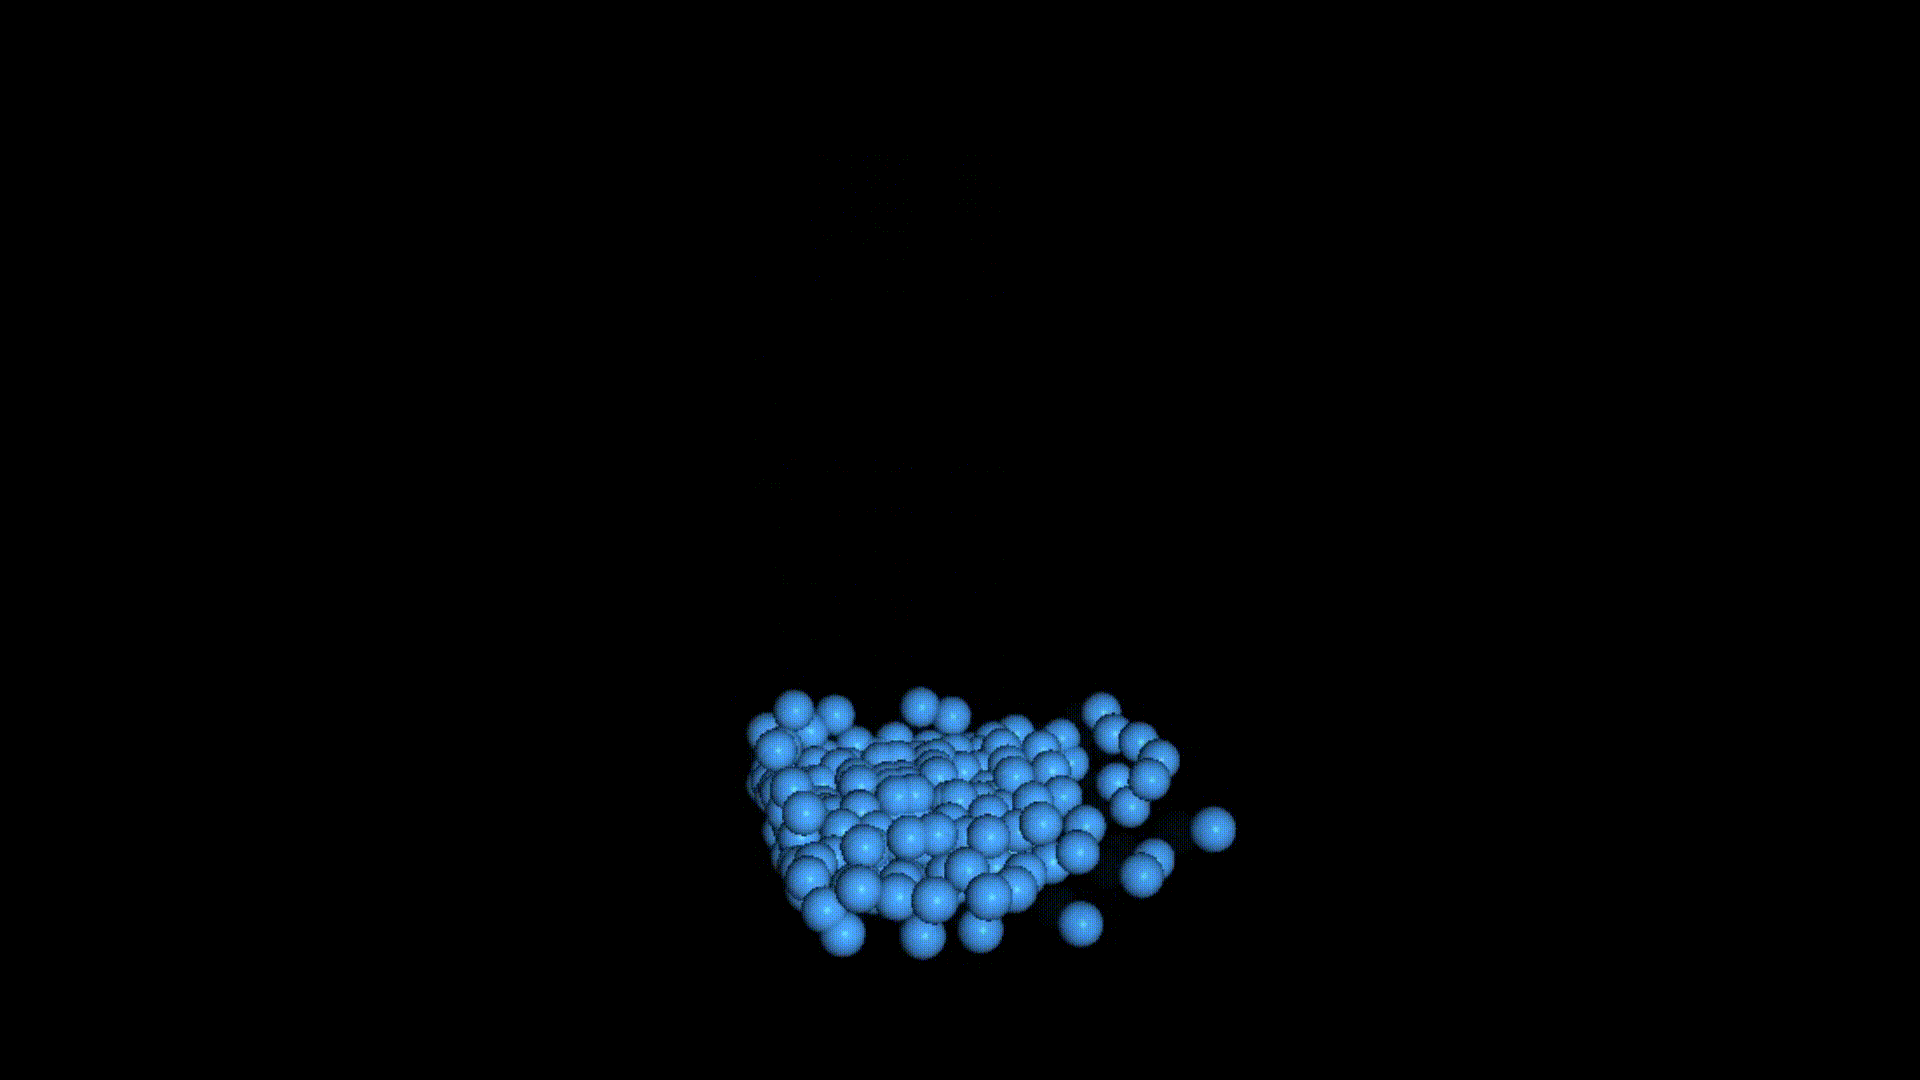
\includegraphics[scale=0.05]{image/image-4.png}
		\end{minipage}
	}
	\subfigure[]
	{
		\begin{minipage}[b]{.4\linewidth}
			\centering
			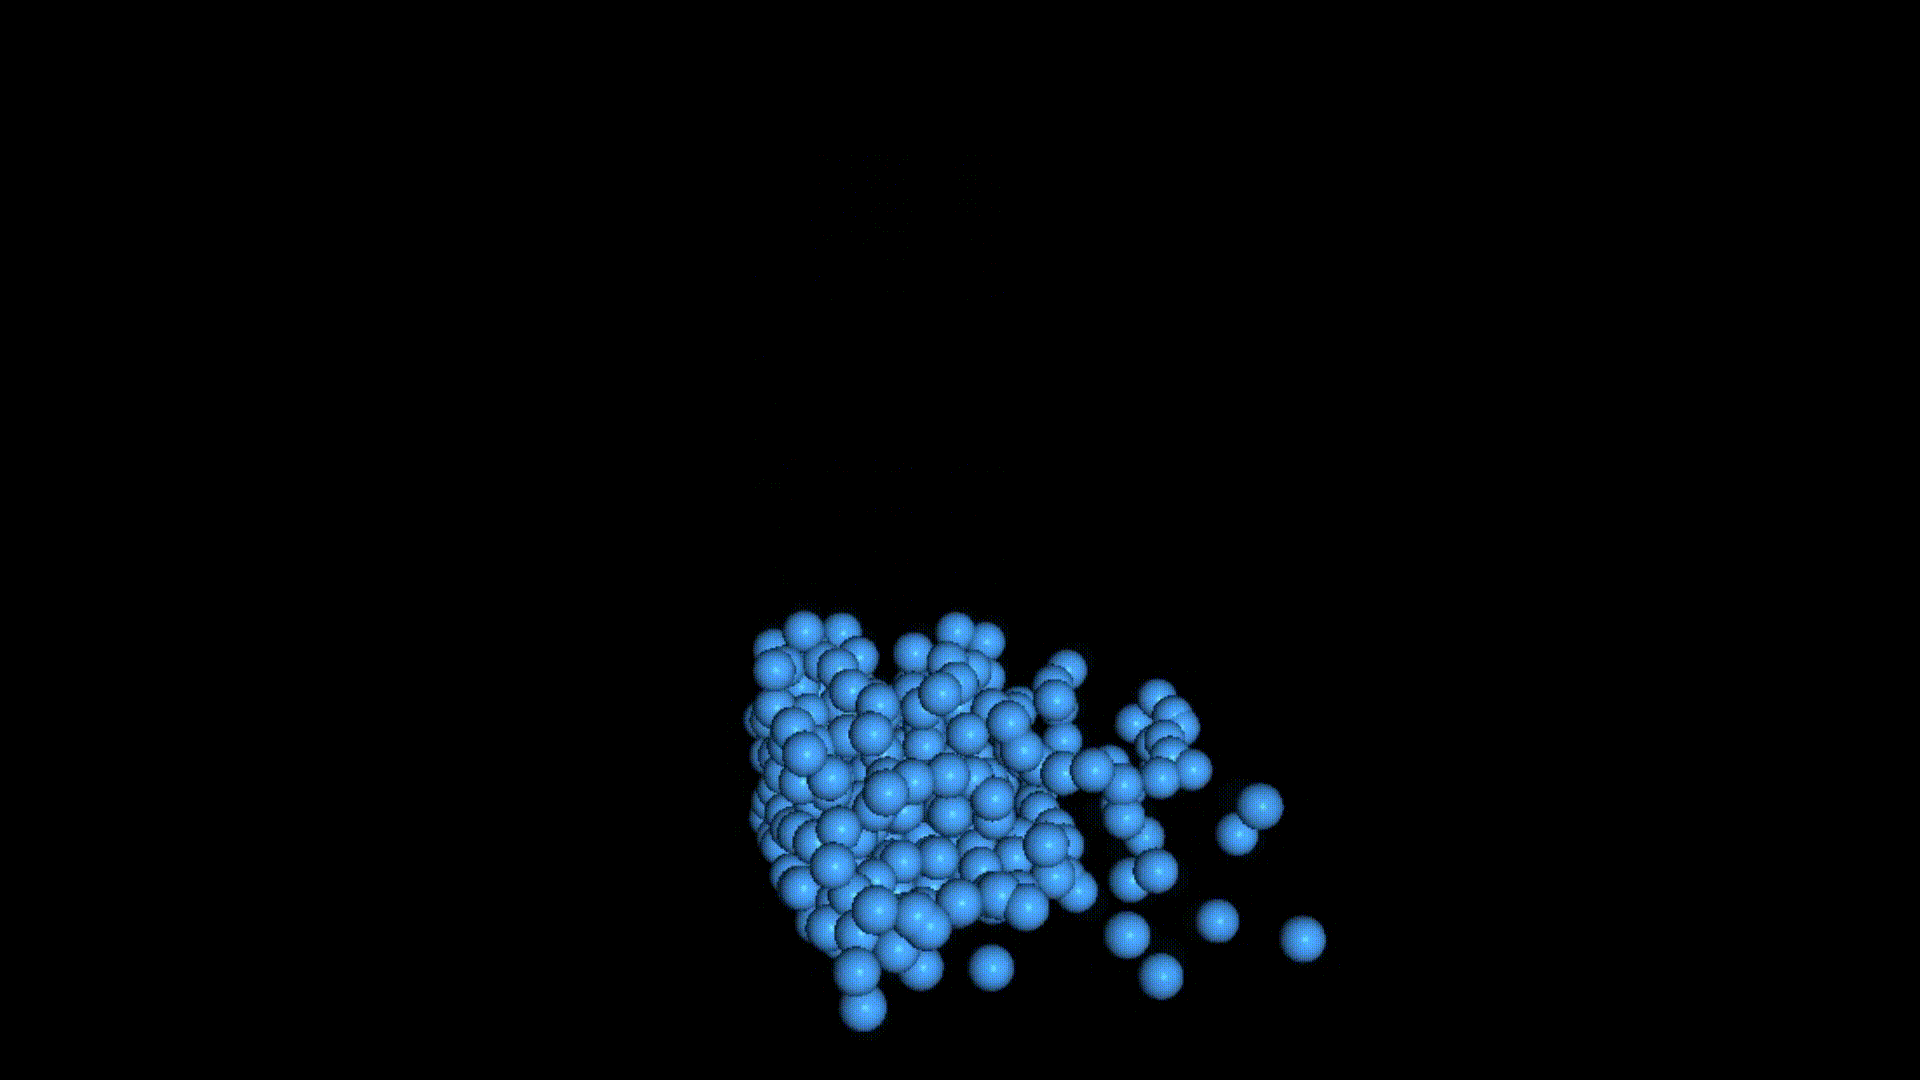
\includegraphics[scale=0.05]{image/image-5.png}
		\end{minipage}
	}
\end{figure}
\begin{figure}[h]
	\centering
	\subfigure[]
	{
		\begin{minipage}[b]{.4\linewidth}
			\centering
			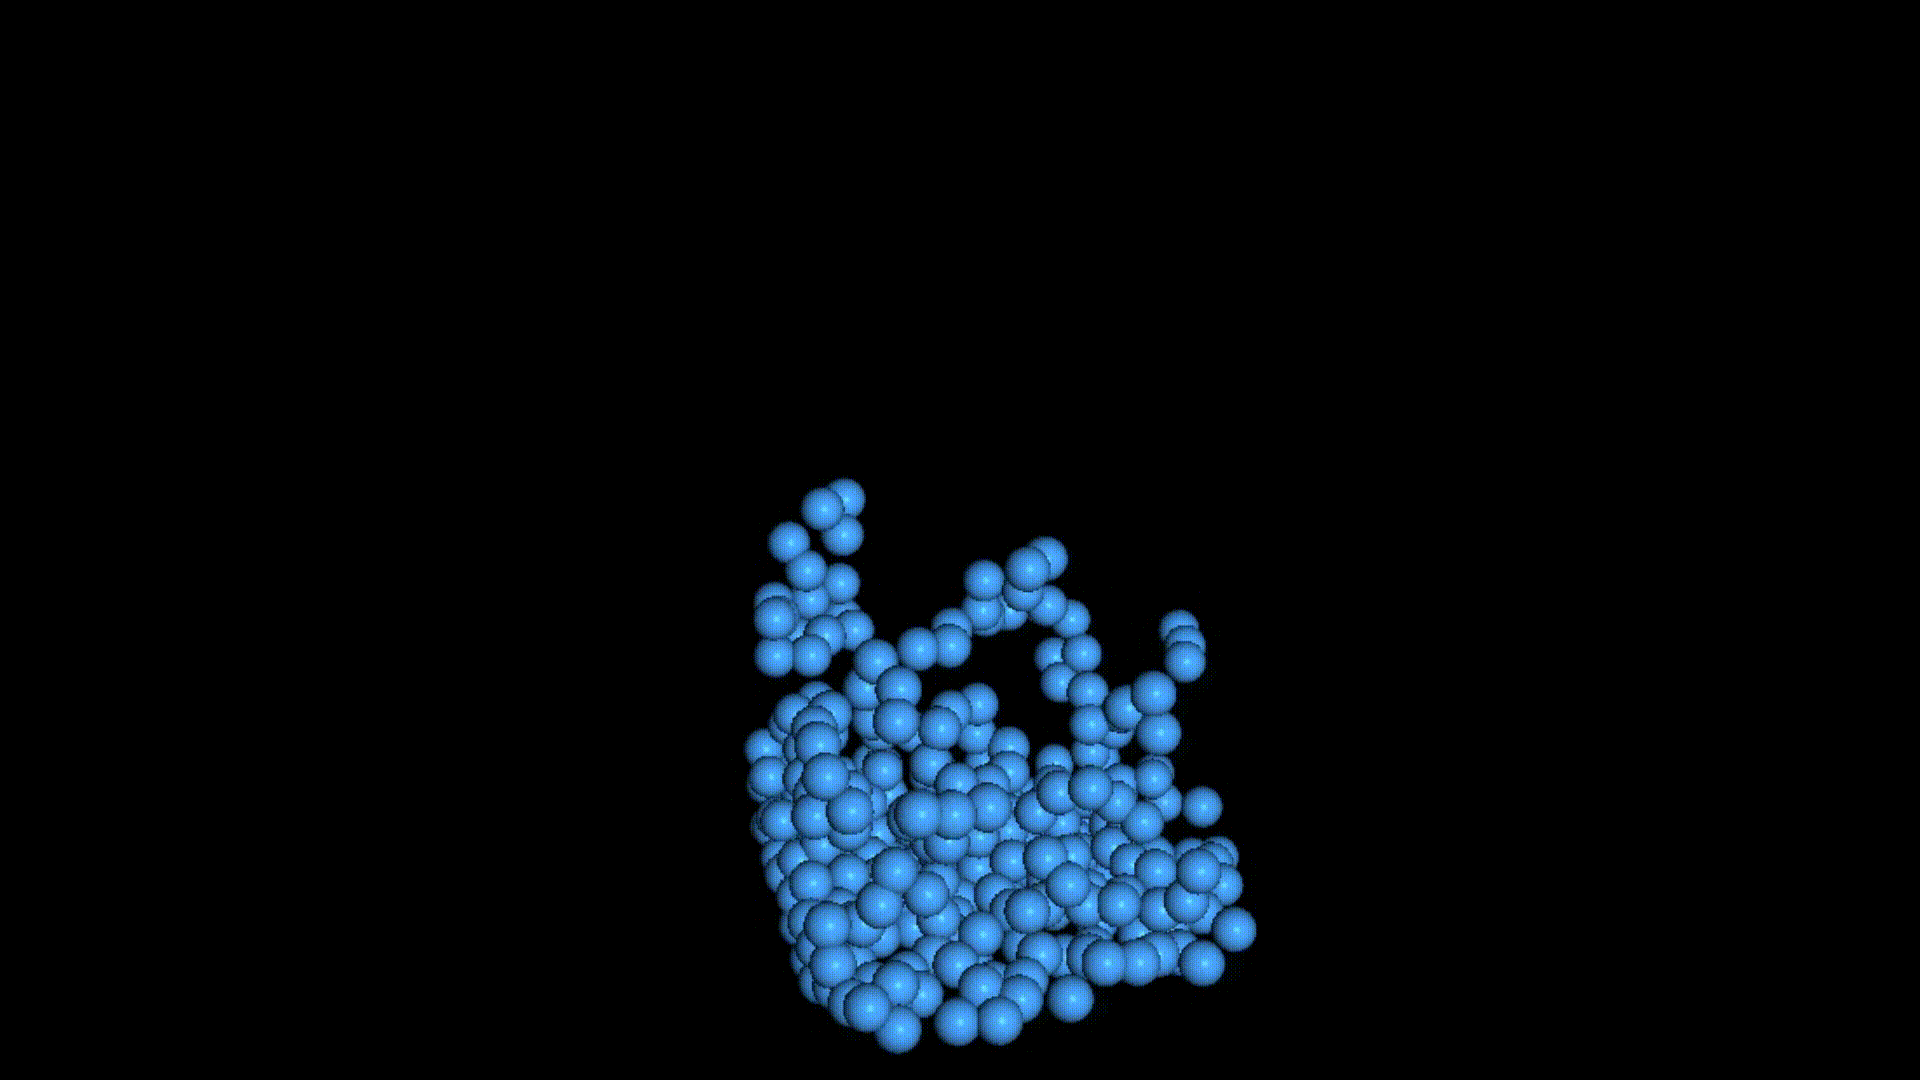
\includegraphics[scale=0.05]{image/image-6.png}
		\end{minipage}
	}
	\subfigure[]
	{
		\begin{minipage}[b]{.4\linewidth}
			\centering
			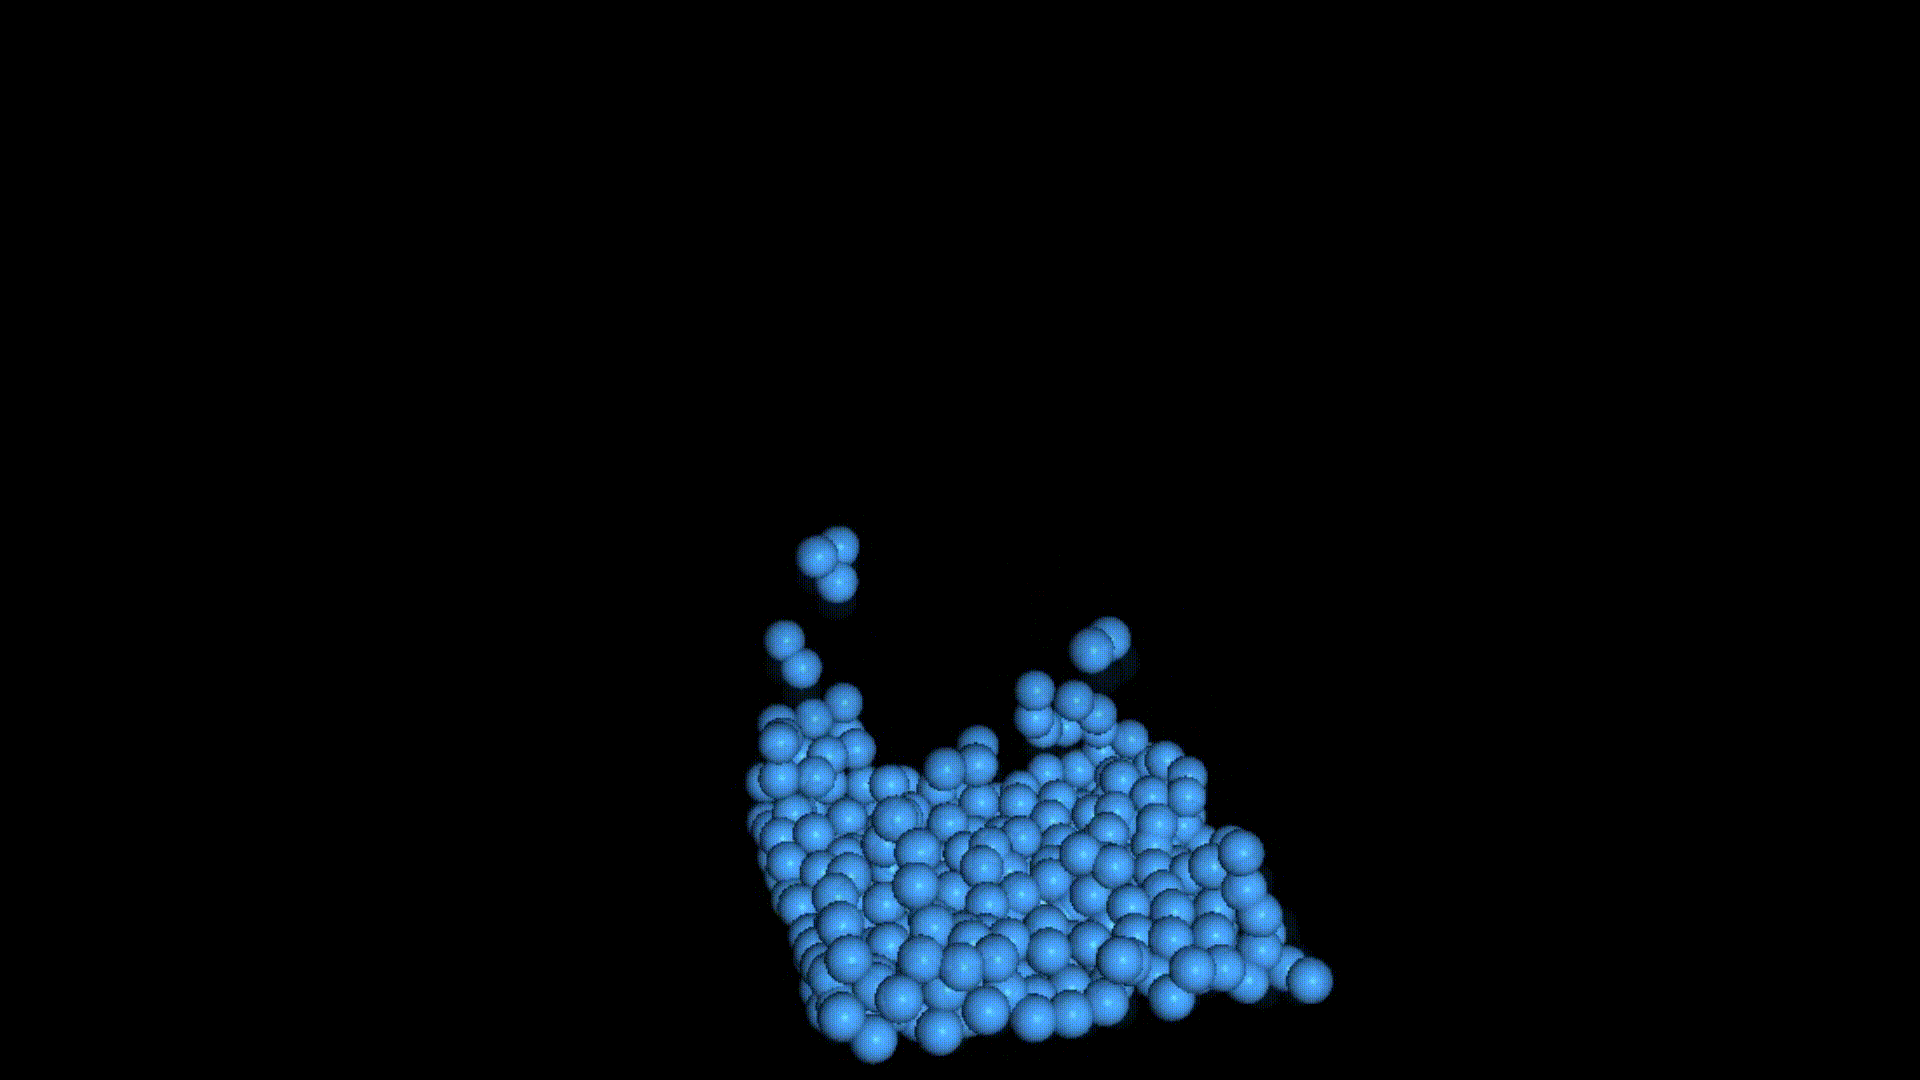
\includegraphics[scale=0.05]{image/image-7.png}
		\end{minipage}
	}
\end{figure}
\begin{figure}[h]
	\centering
	\subfigure[]
	{
		\begin{minipage}[b]{.4\linewidth}
			\centering
			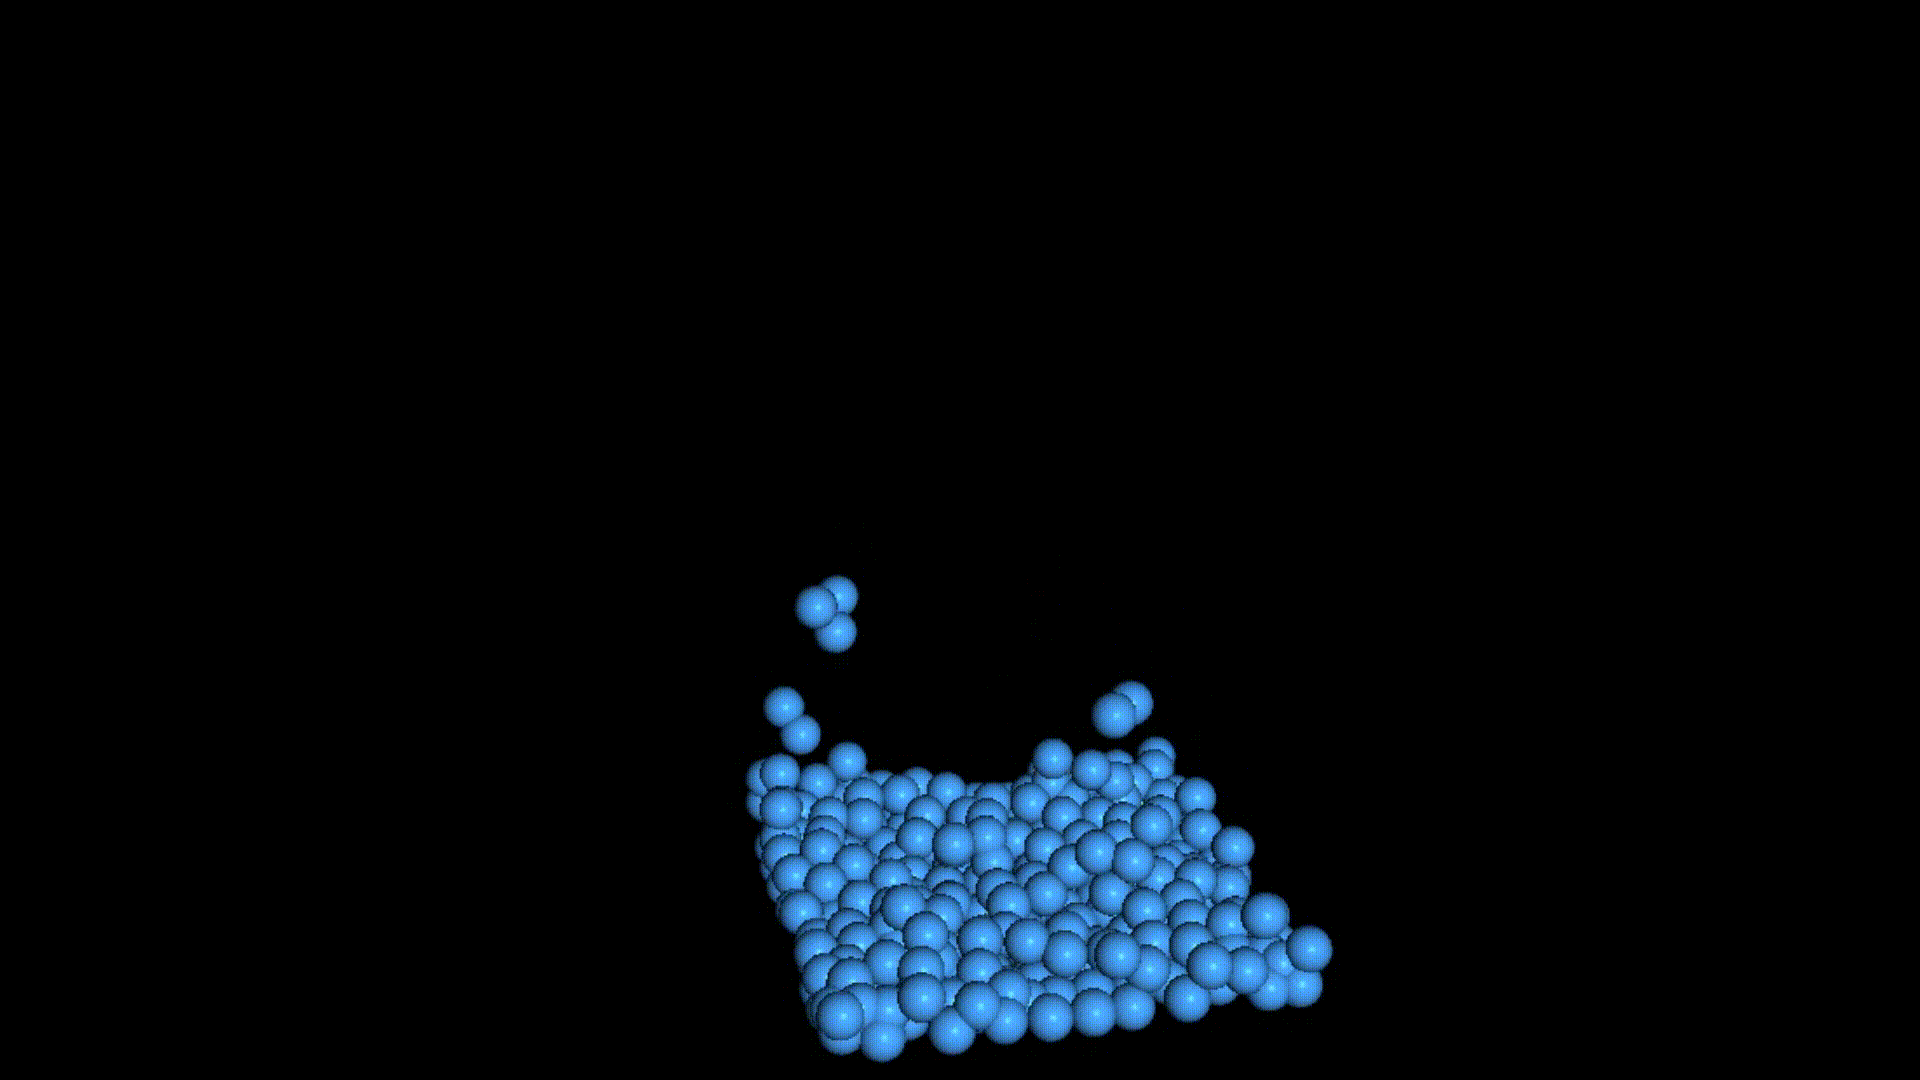
\includegraphics[scale=0.05]{image/image-8.png}
		\end{minipage}
	}
	\subfigure[]
	{
		\begin{minipage}[b]{.4\linewidth}
			\centering
			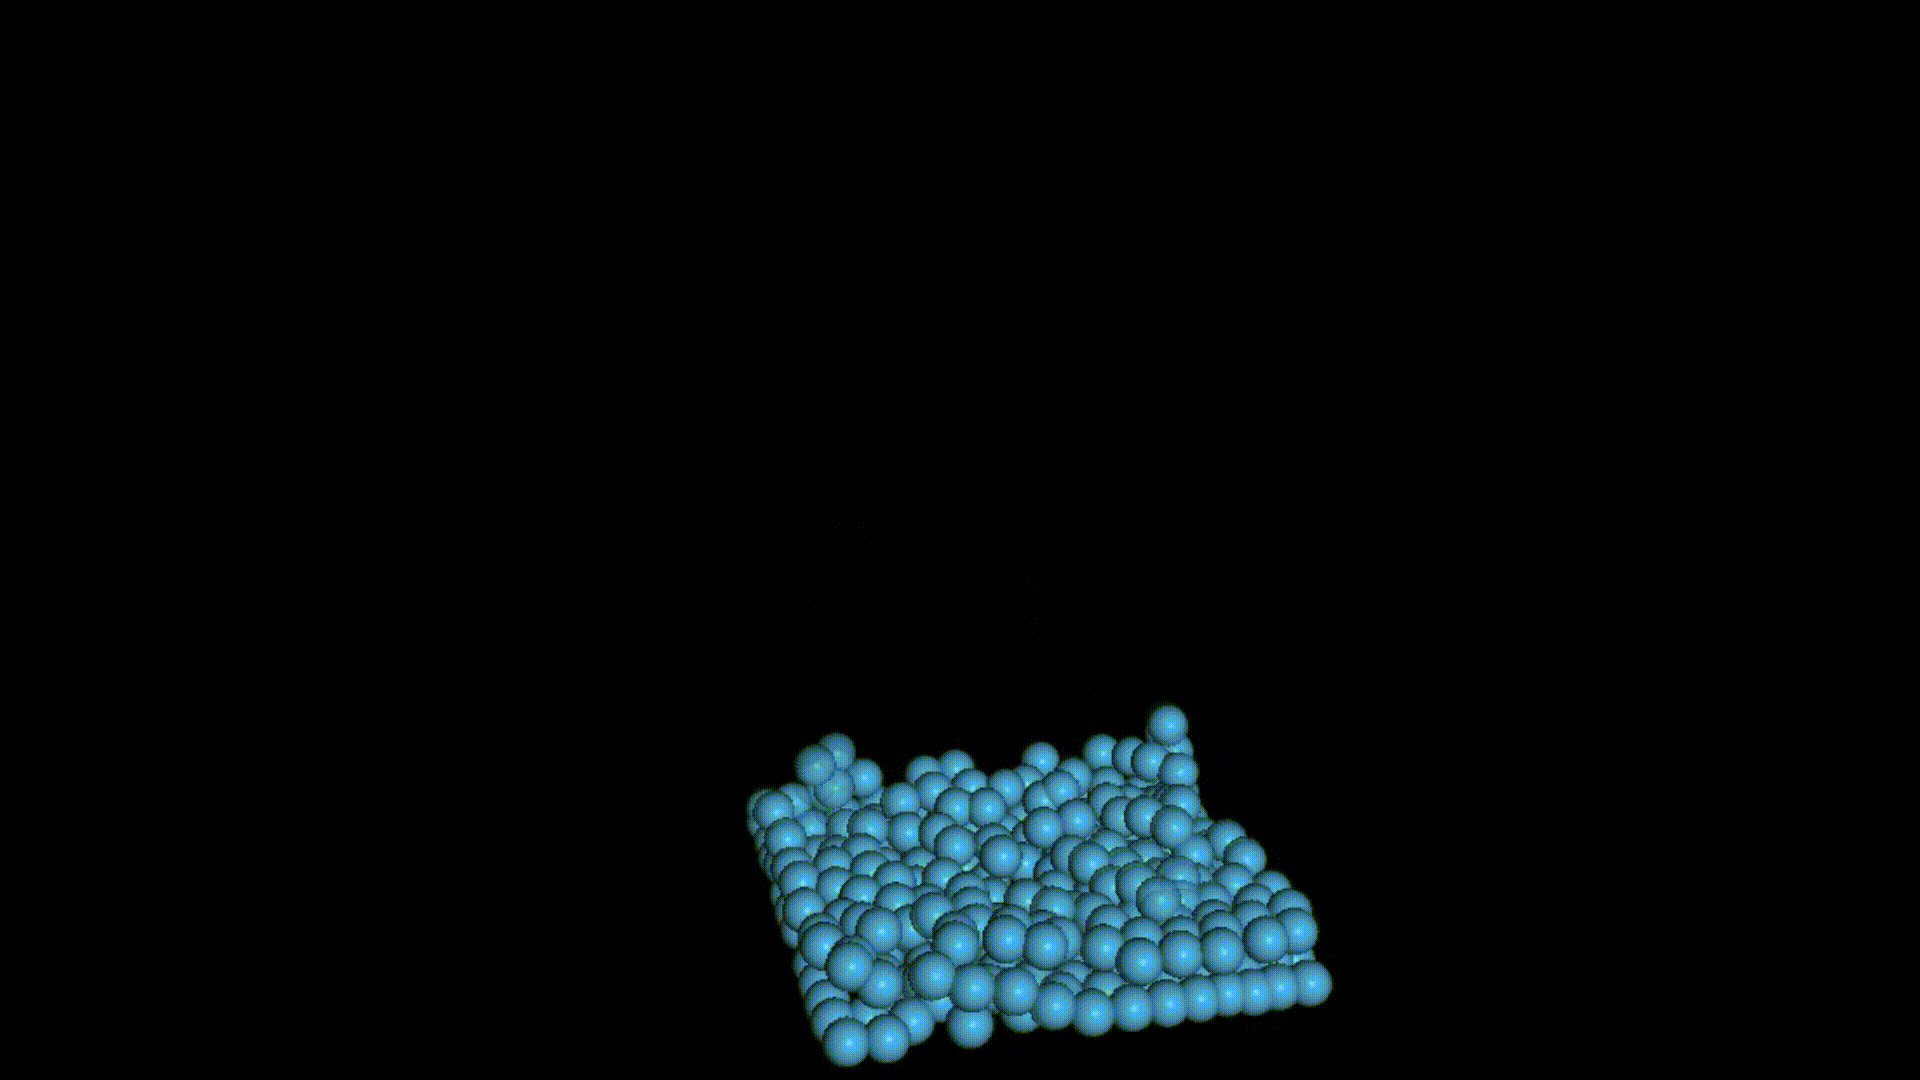
\includegraphics[scale=0.05]{image/image-9.png}
		\end{minipage}
	}
\end{figure}
\begin{figure}[h]
	\centering
	\subfigure[]
	{
		\begin{minipage}[b]{.4\linewidth}
			\centering
			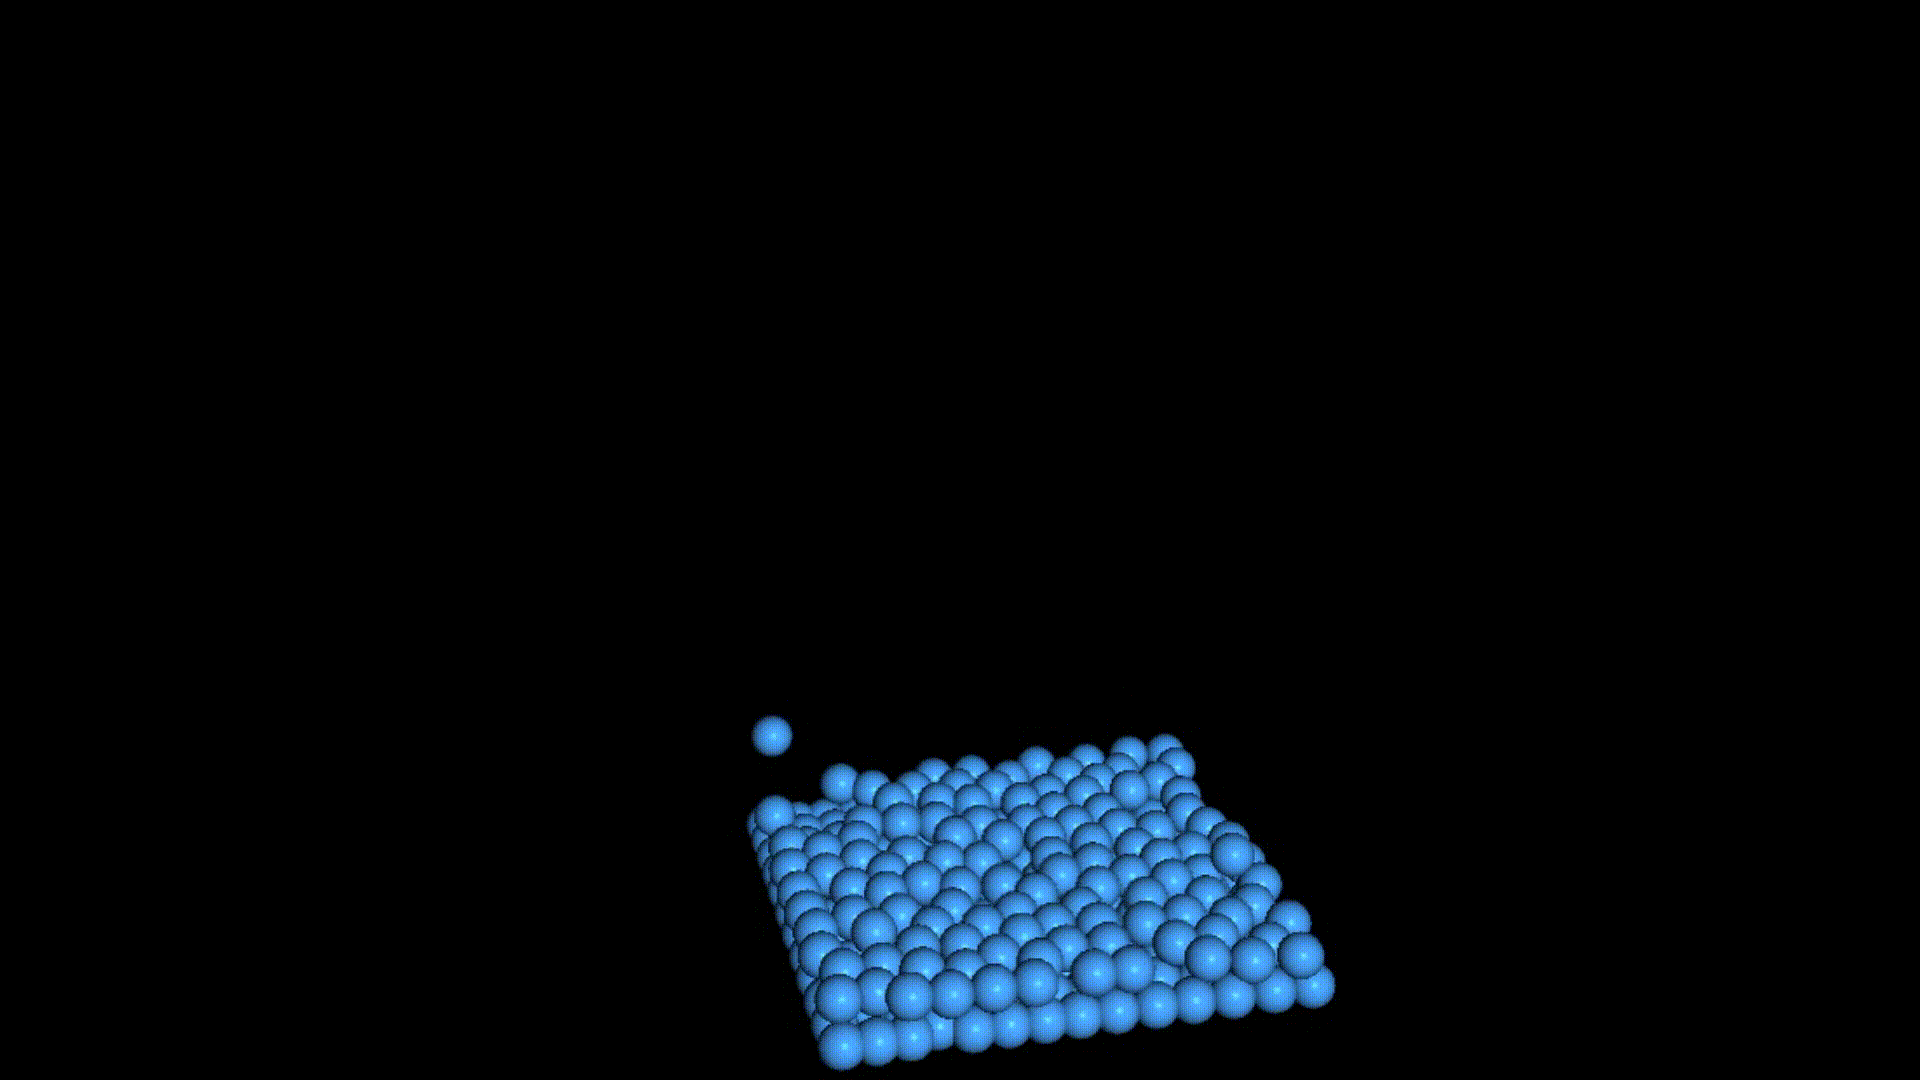
\includegraphics[scale=0.05]{image/image-10.png}
		\end{minipage}
	}
	\subfigure[]
	{
		\begin{minipage}[b]{.4\linewidth}
			\centering
			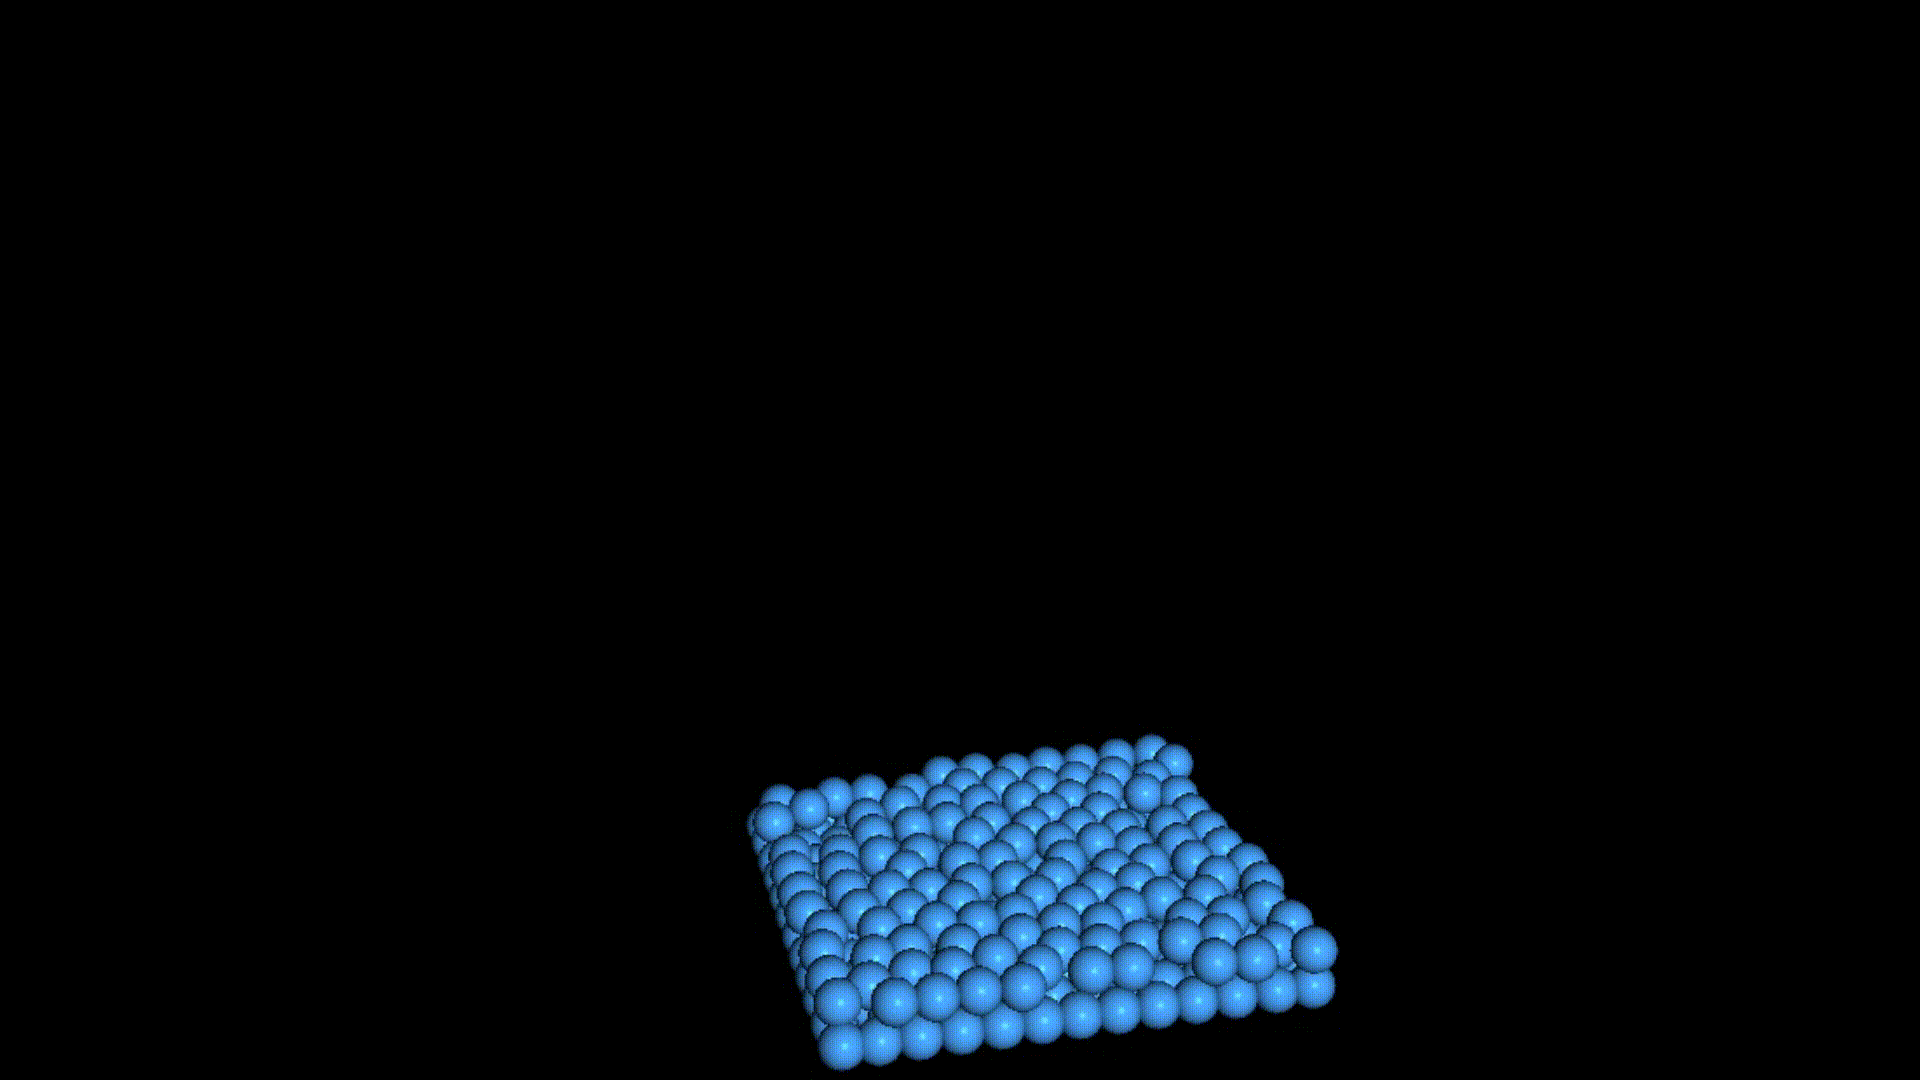
\includegraphics[scale=0.05]{image/image-11.png}
		\end{minipage}
	}
	\caption{status at different time}
\end{figure}


\section{Division of labor}
Yin Hairui handled the most part of programming and the presentation, while Huang Kuan handled some part of programming, the report and made the presentation slides. Both team members participated in the discussion of the main idea and the main process of the project.

\end{document}
